\documentclass[footheight=2em]{beamer}
\usetheme[hideothersubsections]{Hannover}
\usepackage[T1]{fontenc}
\usepackage[utf8]{inputenc}
\usepackage{amssymb}
\usepackage{amsthm}
\usepackage{amsmath}
\usepackage{color,graphicx}
\usepackage{gensymb}
\usepackage{tikz}

\usecolortheme{dolphin}

\title{Projet avion mineure AVI}
\author{Damien Thoral, Gabriel Hondet, Benoit Viry, Nicolas Soulard}
\date{\today}

% ----------------------------------------------------------
% nuremotation des pages -----------------------------------
% ----------------------------------------------------------
\def\swidth{1.6cm}
\setbeamersize{sidebar width left=\swidth}
\setbeamertemplate{sidebar left}
{%
  {\usebeamerfont{title in sidebar}
    \vskip1.5em
    \usebeamercolor[fg]{title in sidebar}
    \insertshorttitle[width=\swidth,center,respectlinebreaks]\par
    \vskip1.25em
  }
  {
    \usebeamercolor[fg]{author in sidebar}
    \usebeamerfont{author in sidebar}
    \insertshortauthor[width=\swidth,center,respectlinebreaks]\par
    \vskip1.25em
  }
  \hbox to2cm{\hss\insertlogo\hss}
  \vskip1.25em
  \insertverticalnavigation{\swidth}
  \vfill
  \hbox to2cm{\hskip0.6cm\usebeamerfont{subsection in
      sidebar}\strut\usebeamercolor[fg]{subsection in
      sidebar}\insertframenumber /\inserttotalframenumber\hfill}
  \vskip3pt
}
% ----------------------------------------------------------


\begin{document}

\frame{\titlepage}

\AtBeginSection[]
{%
  \begin{frame}
    \frametitle{Plan}
    \tableofcontents[currentsection]
  \end{frame}
}

\section{Spécifications}
\begin{frame}[t]{Entrées sorties}
  \begin{scriptsize}
    \begin{figure}
      \centering
      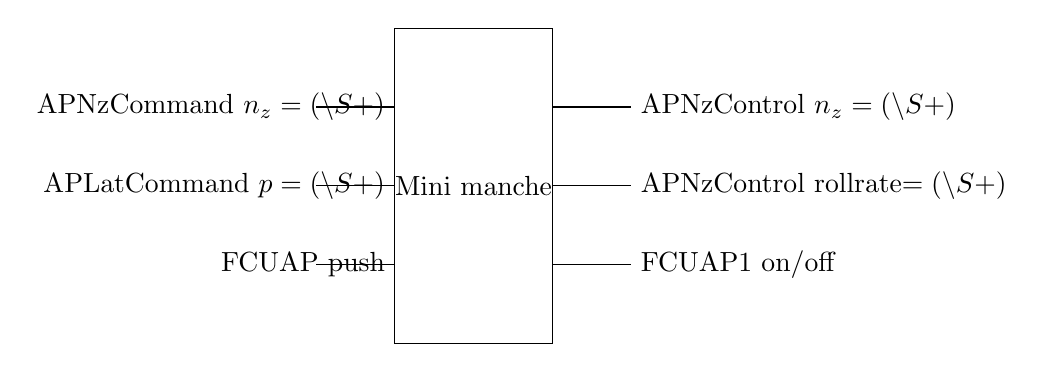
\begin{tikzpicture}
        \draw (0,4) rectangle (2,0);
        \draw (1,2) node {Mini manche};
        % Input
        \draw (-1,1) -- (0,1) node[left] {FCUAP push};
        \draw (-1,2) -- (0,2) node[left] {APLatCommand $p=(\backslash S+)$};
        \draw (-1,3) -- (0,3) node[left] {APNzCommand $n_z=(\backslash S+)$};
        %Output
        \draw (2,3) -- (3,3) node[right] {APNzControl \(n_z=(\backslash S+)\)};
        \draw (2,2) -- (3,2) node[right]
        {APNzControl rollrate\(=(\backslash S+)\)};
        \draw (2,1) -- (3,1) node[right] {FCUAP1 on/off};
      \end{tikzpicture}
      \caption{Entrées et sorties du minimanche}
      \label{fig:io}
    \end{figure}
  \end{scriptsize}
\end{frame}

\section{Boucle de scrutation}
\begin{frame}[t]{Boucle de scrutation}
  \begin{block}{Déclenchement}
    Lancée à chaque réception d'un message de la part de l'auto pilote.
  \end{block}

  \begin{block}{Contenu}
    \begin{enumerate}
      \item mise à jour état du mini manche (actif ou non)
      \item si actif, lecture des données provenant du mini manche
      \item vérification de la valeur (saturation)
      \item renvoit de la valeur sur le bus.
    \end{enumerate}
  \end{block}

  \begin{block}{Distinction des grandeurs}
    Une boucle ne concerne qu'une seule grandeur (\(n_z\) ou \(p\)),
    déterminée par le message la déclenchant.
  \end{block}
\end{frame}

\section{Gestion des événements entrants}
\subsection{Module \texttt{pygame}}
\begin{frame}[t]{Module \texttt{pygame}}
  \begin{block}{File d'événements}
    Une file contenant tous les événements provenant du mini manche est
    maintenue par \texttt{pygame}.
  \end{block}
  \begin{block}{Interaction avec la file}
    \begin{itemize}
      \item \texttt{get()} renvoit les données du minimanche et vide la file.
      \item \texttt{get(evt)} ne traite que les événements du type \texttt{evt}.
    \end{itemize}
  \end{block}
\end{frame}

\subsection{Gestion des événements}
\begin{frame}[t]{Gestion de la file}
  \begin{block}{Données}
    Chaque grandeur dispose
    \begin{itemize}
      \item d'une liste contenant toutes les entrées depuis la dernière boucle
        la concernant,
      \item une variable \texttt{LASTAXISV} contenant la dernière
        valeur relevée.
    \end{itemize}
  \end{block}
  \begin{block}{Obtention des données}
    \begin{enumerate}
      \item La file d'événements est vidée dans une liste temporaire,
      \item les événements de la file temporaire sont répartis entre les listes
        correspondant aux grandeurs,
      \item la variable \texttt{LASTAXISV} correspondante est modifiée, et sa
        valeur est renvoyée.
    \end{enumerate}
  \end{block}
\end{frame}

\begin{frame}[t]{Gestion de l'auto pilote}
  \begin{block}{Besoin de thread}
    L'appui de boutons pour désactiver l'auto pilote devant être effectif à tout
    moment, un thread dédié est nécessaire.
  \end{block}
  \begin{block}{Contenu du thread}
    Boucle infinie appelant la procédure \texttt{update\_ap},
    \begin{enumerate}
      \item récupérer l'état du pilote automatique via une variable
        globale,
      \item récolter des événements de la file concernant les appuis boutons,
      \item si un bouton a été pressé et que le pilote n'était pas enclenché,
        alors désenclencher le pilote automatique,
      \item renvoyer l'état de l'auto pilote.
    \end{enumerate}
  \end{block}
\end{frame}

\subsection{Traitement des données}
\begin{frame}[t]{Plages de valeurs}
  \begin{block}{Définition des plages}
    \begin{itemize}
      \item \(n_z \in \mathbf{D}_{n_z} = [-1, 2.5]\)m\(\cdot\)s\(^{-2}\),
      \item \(p \in \mathbf{D}_p = [-15, 15]\deg\cdot\)s\(^{-1}\).
    \end{itemize}
  \end{block}
  \begin{block}{Conformité des données}
    \begin{itemize}
      \item Si auto pilote activé, les données passent par une
        fonction \(f\colon D \mapsto \mathbf{D}_{n_z}\) ou \(\mathbf{D}_p\),
      \item sinon, une fonction \(g\colon[-1, 1] \mapsto \mathbf{D}_{n_z}\) ou
        \(\mathbf{D}_p\) associe à la valeur en sortie du mini manche une valeur
        adéquate.
    \end{itemize}
  \end{block}
\end{frame}


\section{Tests}
\begin{frame}[t]{Définition des tests}
  \begin{block}{Valeurs de test}
    Envoi d'une série de 10 valeurs aléatoires au mini manche,
    \begin{itemize}
      \item \(n_z \in [-5, 5]\),
      \item \(p \in [-30, 30]\).
    \end{itemize}
  \end{block}
  \begin{block}{Test de valeurs}
    Vérification de la conformité des valeurs en sortie,
    \begin{itemize}
      \item \(n_z \in [-1, 2.5]\),
      \item \(p \in [-15, 15]\).
    \end{itemize}
  \end{block}
  \begin{block}{Boucle temporelle}
    Envoi d'une valeur de \(n_z\) et de \(p\) à chaque boucle temporelle.
  \end{block}
\end{frame}

\begin{frame}[t]{Résultats des tests}
  \begin{block}{Valeur envoyée dans l'intervalle admissible}
    \begin{enumerate}
      \item Comparaison entre la valeur envoyée et la valeur reçue,
      \item \texttt{True} si les deux valeurs sont identiques, \texttt{False}
        sinon.
    \end{enumerate}
  \end{block}
  \pause
  \begin{block}{Valeur envoyée inférieure à la valeur minimale (resp.\
      maximale) admissible}
    \begin{enumerate}
      \item Comparaison valeur reçue et valeur minimale (resp.\ maximale)
        admissible,
      \item \texttt{True} si égalité, \texttt{False} sinon.
    \end{enumerate}
  \end{block}
  \pause
  \begin{block}{Saturation}
    Lorsque les valeurs sont hors de l'intervalle admissible, le mini manche doit
    renvoyer la borne la plus proche de l'intervalle.
  \end{block}
\end{frame}

\section*{Bilan}
\begin{frame}[c]{Bilan}
  \begin{block}{Safety nets}
    Implémentés mais non fonctionnel à cause du vecteur d'état.
  \end{block}
  \begin{block}{Améliorations}
    Ergonomie améliorable, e.g.\ relation non linéaire entre l'angle du
    mini manche et la consigne.
  \end{block}
\end{frame}
\end{document}
